

\chapter{Introduction}

%\label{chap:GettingStarted}
\section{Overview}
                     
Dark matter is among the most fascinating and enigmatic features of the universe. Although representing roughly 27\% of the mass-energy content in the universe, this composition has yet to be detected directly.\cite{planck2016} Unlike normal matter, which feels electromagnetic forces, dark matter does not emit, absorb, or reflect light so it cannot be viewed using telescopes. Attendant necessarily to such a particle of "dark" matter would be the creation of theories to account for all the rest of what we observe without it. Its existence was first proposed in the early 20th century, as it had become apparent that visible material alone could not explain all the observed motion of galaxies and galaxy clusters.

Dark matter is detected and analyzed indirectly through gravitational effect on visible matter, which includes its influence upon the motion of galaxies and stars, accelerating the universe's flow in space-time (also cutting forth its mass content), acting as a bendable mass source for gravitation lensing, and merging corpuscular small-scale elements into large-scale structures. One of the most potent evidence for dark matter arises from the fact that galaxies spin far more rapidly than can be explained by their visible content alone.\cite{rubin1970} This indicates an immense amount of invisible mass is exerting extra gravitational force, and thereby preventing galaxies from flying apart.

Dark matter has not yet been directly observed, but its composition is assumed to be the same that of matter that does absorb radiation like light. The more promising sought-after dark matter particles are WIMPs, axions, or sterile neutrinos, none of which have been observed experimentally yet.

Astrophysics and cosmology have made dark matter a very hot topic in recent years with many theories and models being proposed. Scientists want to learn about its properties, where it is located and how it interacts with “ordinary” visible matter, which could have broad implications regarding the structure and evolution of everything in the universe. Machine learning (ML) methods have lately shown the potential to effectively process multiple sources of cosmological data, recognize patterns, and make inference about the behavior and properties of DM in a manner that opens up new paths for investigation of this elusive entity.

 
\begin{figure}[H]
    \centering
    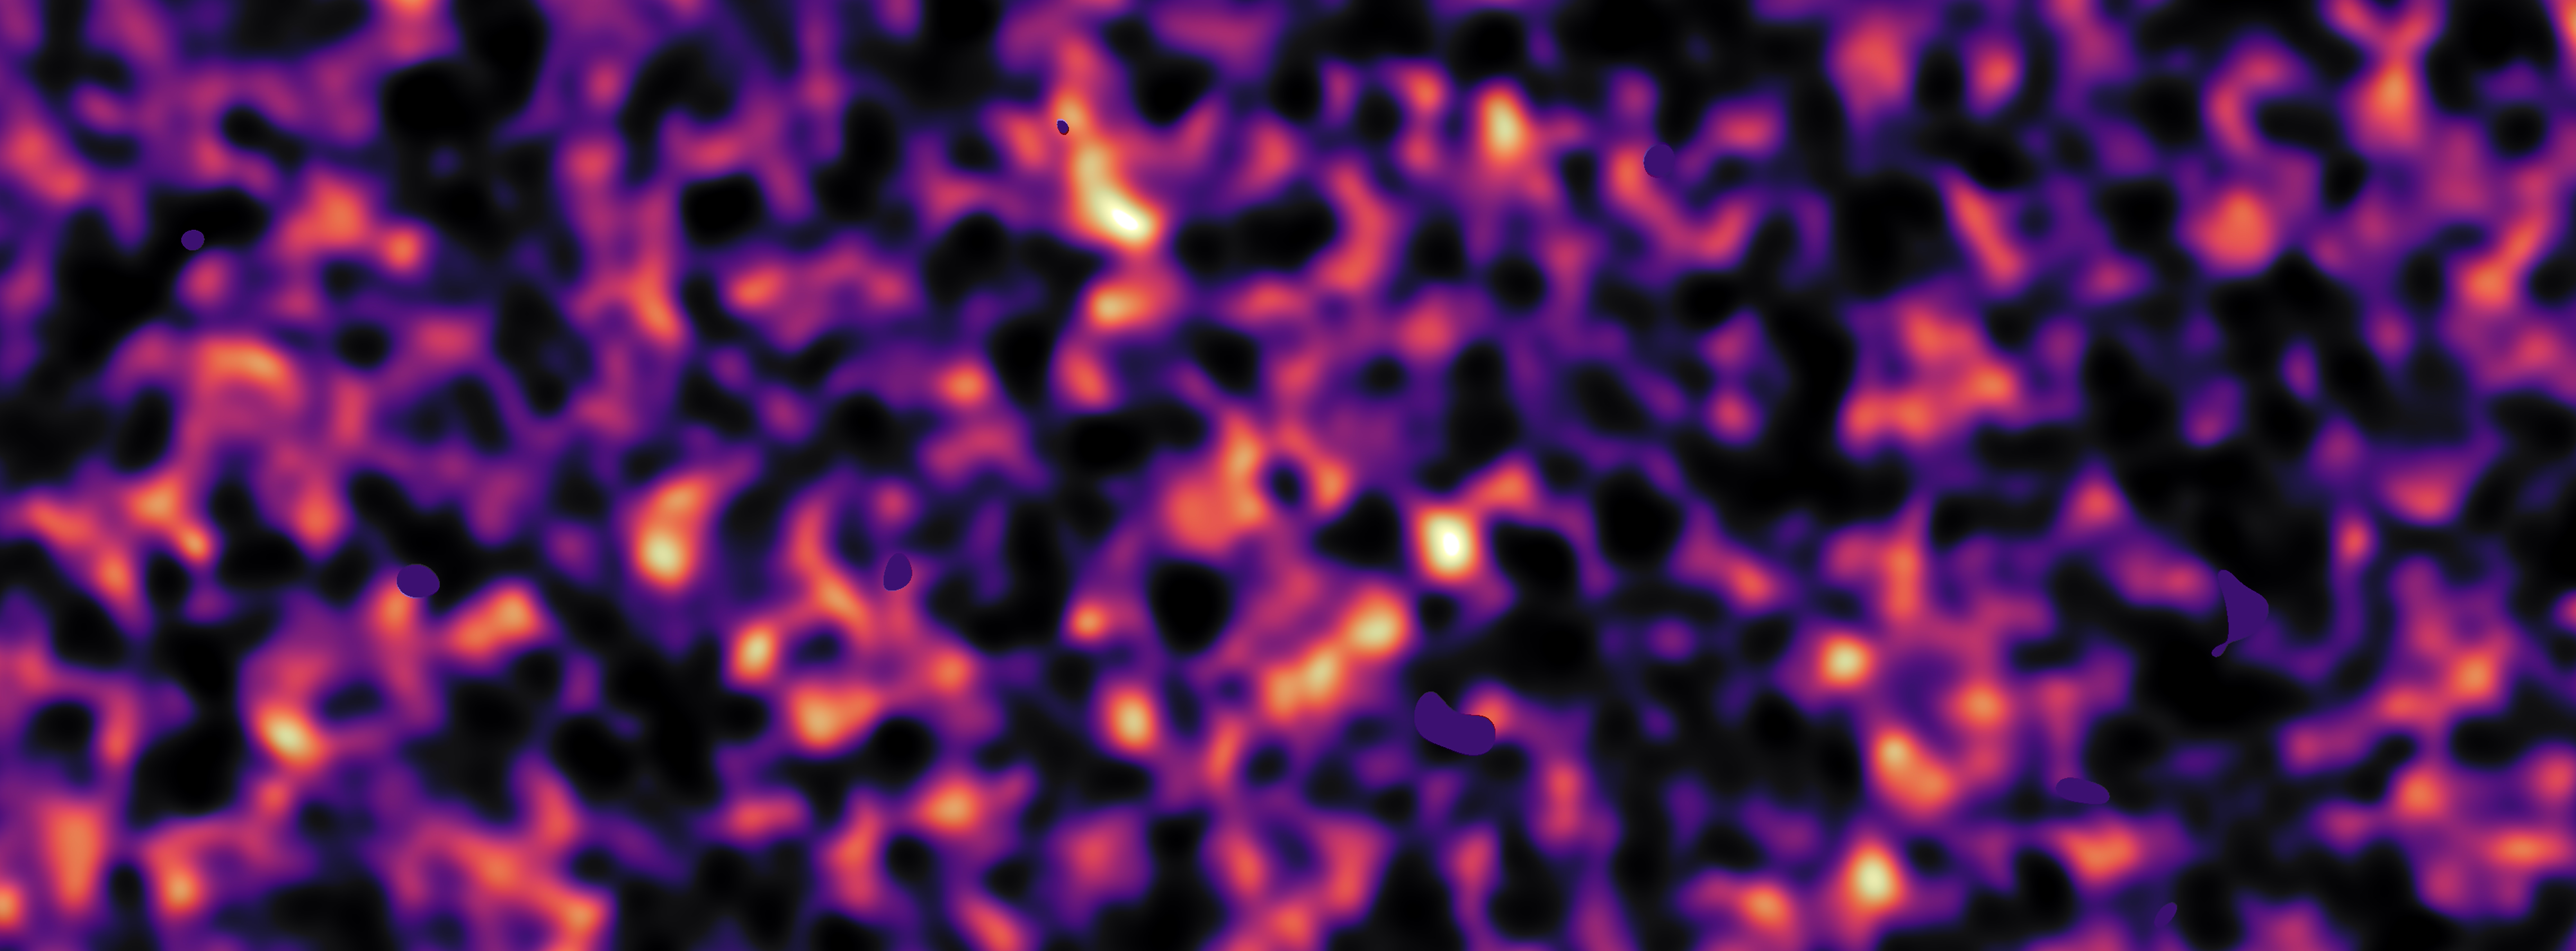
\includegraphics[width=1\linewidth]{Chap1/dark_matter_map.jpg}
    \caption{Dark matter map for a patch of sky based on gravitational lensing analysis of a Kilo-Degree Survey \cite{wikiDM}} 
    \label{fig:enter-label}
\end{figure}





\subsection{Observational Tests of the Dark Matter Scenario }  
Despite being invisible, dark matter has a substantial gravitational pull on visible matter and therefore numerous astrophysical observations have helped establish the existence of dark matter. A key early indication comes from observing the rotation curves of galaxies. According to Newtonian mechanics, stars and gas orbiting in a galaxy should slow down the farther they get from its center, where less mass is concentrated. But when we turn to observations of spiral galaxies, we find that stars at their outskirts are spinning, but they’re spinning far too quickly considering all the mass we can account for by the light produced from them. That implies the existence of more, unseen mass tugging on it gravitationally, a form of matter known as dark matter. The existence of this unseen mass, commonly known as the "dark halo," is required to account for both the observed flat rotation curves and the differences between predicted and actual stellar velocities within galaxies.

The Legacy of Gravitational Lensing is also a vital line of evidence for general relativity, the gravitational bending of light that Einstein’s 100-year-old theory predicts. When a beam of light from a very distant object such as a galaxy passes close to something big, like another galaxy cluster (or other matter of lesser mass), the path of that light beam gets bent and distorted, and you get warped looking images of background objects. The magnitude of this effect is directly related to the mass of the lensing body. Measurements of gravitational lensing around galaxy clusters provide evidence that the mass indicated by the lensing is much larger than that comprised only of visible matter contained in such clusters, implying that dark matter exists. One of the best known cases, the Bullet Cluster, has a separation between visible (X-ray) and dark matter (inferred from lensing), providing even more striking evidence for dark matter in galaxy clusters.\cite{clowe2006}

Evidence for dark matter The Big Bang left behind the Cosmic Microwave Background (CMB). These differences are those of temperature fluctuations of the CMB, which in turn reflect small density variations in the matter content and distribution of the early universe. These fluctuations are what enables cosmologists to infer the distribution of visible and invisible matter at that time. The results from the CMB, in particular the angular scale subtended by the first acoustic peak, provide extensive evidence for dark matter. Dark matter was essential for the gravitationally driven growth of cosmic structure that is encoded in the fluctuations in the CMB. By observing these fluctuations, researchers have measured the quantity of dark matter in the universe and verified its vital role in defining the cosmos.

Taken together, these three observational facts— galaxy rotation curves, gravitational lensing and Cosmic Microwave Background are a compelling suite of evidence for the reality of dark matter. Not only do they show that dark matter is critical for the creation of galaxies and galaxy clusters they also offer clues on what role it played in the early universe.

 

\subsection{Early Dark Matter Theories } 


It was around the early 20th century that scientists first began to realize that there were discrepancies between the motion of cosmic objects as they observed it and how much visible matter they could count. First evidence of what would eventually become known as dark matter comes from the research of the rotation curves of galaxies and member galaxy motions in clusters.

In 1933, the Swiss astronomer Fritz Zwicky observed one of the first pieces of evidence with dark matter. While observing the Coma galaxy cluster, Zwicky realized that galaxies in a cluster were moving at much higher velocities than could be explained by the matter we could see.\cite{zwicky1933} In terms of classical Newtonian mechanics, the gravitational attraction of the visible matter in the cluster should have decelerated the motions of galaxies and dispersed them until they could eventually escape from the cluster. But Zwicky’s measurements revealed that the total mass of the cluster didn’t suffice to explain what was keeping the galaxies tied up. He posited that there was a mysterious force of otherwise undetectable “missing mass” which was just sufficient to bind the galaxies. This “missing mass” would foreshadow the modern idea of dark matter. Zwicky even went so far as to call the substance “dunkle materie” or dark matter, although the idea went mostly unheralded at the time.\cite{zwicky1933}

The idea received a boost in the 1970s after astronomer Vera Rubin, building on Zwicky’s research, analyzed the rotation curves of galaxies.\cite{rubin1970} Rubin and her colleague Kent Ford discovered that stars on the outskirts of spiral galaxies were moving at unexpectedly high rates, given only the amount of visible matter in these galaxies. Also like Zwicky, Rubin determined that some type of dark or hidden mass must be exerting gravitational forces upon the stars in the arms, reinforcing her belief in the existence of dark matter. Her work was instrumental in placing dark matter at the center of modern cosmology.

When the notion of dark matter was first proposed, it originated from our inability to explain the motions of galaxies (as well as galaxy clusters) using gravity and regular baryonic matter alone, and scientists were free to imagine what kind of form this mysterious missing mass could take. It was speculated by some that it could be made up of ordinary, invisible or “dark” matter like faint stars or clouds of gas (so-called baryonic matter). But None of these is consonant with all the observed facts, notably the large structure of universe and detailed dynamics of galaxy clusters.

As dark matter was better understood, it turned out that it couldn’t just be regular old matter. This, in turn, eventually gave rise to the more sophisticated theories that exist today which postulate cosmological dark matter is primarily made of non-luminous, non-interacting particles. These particles (which interact via gravitational and, potentially, the weak force) give rise to more distinctive dark matter theories such as WIMPs and axions that will be discussed later in the section.

So, that's an overview of the early theories of dark matter which were developed mostly in response to astronomical data on galaxy and cluster motion. Zwicky and Rubin’s work helped establish the modern conception of dark matter as an essential part of the mass that makes up the universe, but what dark matter actually is would remain a mystery for decades.

 
 
\section{Problem Statement}
 The identification and characterization of dark matter are among the key open problems in astrophysics today. Novel approaches are required to overcome the absence of direct observational data. Machine learning can help us digest large complex datasets, allowing us to predict the properties and behaviors of dark matter. The goal of this proposal is to study the applicability of ML techniques on dark matter-related data and where possible discover new patterns/anomalies that would proof for such a distributed substance.

 

 
\subsection{Data Acquisition:}

In dark matter studies, the data acquisition is the essential part for collecting evidences to interpret this unknown and cold component of the universe. A spider web of cosmic proportions Because dark matter can’t be sensed directly, scientists employ a range of indirect means to gather information that might shed light on its existence, distribution and behavior. Such data are collected through astronomical observatories, space missions and with experiments aimed to detect the influences that dark matter has on visible materials and light.


Most of the data gathering in dark matter studies uses information from astronomy. Observations of galaxies, galaxy clusters and the like are needed to detect how dark matter’s gravitational clout impacts visible matter. Telescopes, on the ground and in space, provide data about how stars, gas and galaxies move. Notable examples include:

Rotation curves of galaxies: Measurements on galaxies rotation speeds that is evidence for dark matter halos. They are typically collected with optical and radio telescopes.

Gravitational Lensing: The deflection of light from faraway galaxies by the gravitational pull of dark matter in galaxy clusters. This is the data collected with optical and infrared telescopes including the Hubble Space Telescope and ESA's Gaia satellite.

Cosmic Microwave Background (CMB) satellite such as the Planck satellite have been measuring CMB-data, which is evidence for the structure of the early universe and how dark matter played a role in influencing its evolution. Temperature fluctuations in the CMB can be used to map matter density in the early universe.



 
\begin{figure}[H]
    \centering
    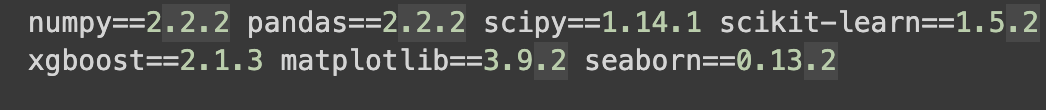
\includegraphics[scale=0.6]{Chap1/libraries.png}
    \caption{Necessary Libraries }
    \label{fig:my_label}
\end{figure}



\section{Motivation}
The origin of dark matter is one the deepest questions in contemporary astrophysics and cosmology. Though postulated to exist, dark matter experiments have so far failed to detect this elusive substance. Observational evidence, such as galaxy rotation curves, gravitational lensing, and the cosmic microwave background indicates that it exists, but its precise nature is still unknown. This difficulty has pushed researchers to investigate new ways for analyzing data, among which ML are one of the most promising.

 



 
\section{Objectives} 
The goal of this effort is to use machine learning algorithms to predict and model various dark matter phenomena. Specific goals include:

\begin{itemize}
    \item To Estimate Dark Matter Distribution: Apply machine learning approaches to large-scale astronomical datasets and predict the spatial distribution of dark matter within galaxy clusters and in other cosmic structures.

    \item To Enhance Detection Sensitivity: Model machine learning algorithms which can enhance the sensitivity of the dark matter detection techniques like gravitational lensing, galaxy rotation curves and direct detection experiments.

    \item To Create Dark Matter Simulation: Develop computational tools that can predict the interactions of dark matter particles (e.g., WIMPs, axions) in different astrophysical environments so as to identify potential dark matter signatures.

    \item To Analyze Gravitational Effects: Analysis the influence of dark matter gravitational effect on visible stuff (e.g., their impact on galaxy motion, galaxy clusters and overall cosmic structures).

    \item To Develop and Enhance Data Analysis Techniques: Enhance techniques for analyzing large, intricate data sets from telescopes, experiments and simulations to identify dark matter signals more quickly and accurately.
\end{itemize}

\section{Scope of Work}
\begin{itemize}

    \item Indirect Evidence: As we cannot detect dark matter directly, the evidence is only indirect and uncertainties in the corresponding predictions of machine learning models may occur.

    \item Quality of data: The reliability of predictions and simulations crucially relies on the quality of observational data. “Negative” or “unlabeled” data: Negative data in unsupervised learning and semi-supervised learning can end up producing inaccurate, biased machine learning results.

    \item Uncertainty about Dark Matter Properties: The study is limited by our current lack of understanding as to the precise nature of dark matter. Machine learning predictions can be speculative without a model to guide them.

    \item Algorithm Complexity: Machine learning learn models with deep feature set can be complex and expensive to compute rendering hard the scaling of the research to a volume of data necessary enough for hypothesis raising results.

    \item Existing model assumptions: Dependence on existing theoretical framework like $\Lambda$-CDM limit the ability to explore alternate dark matter theories and hence might confine the scope of the predictions.

\end{itemize}
\section{Challenges}


\begin{itemize}
    \item Data Processing and Integration: Integrating data from different sources (galaxy surveys, particle detectors, simulations etc) may be difficult when the data is in different formats or are using different measurement technology and spatial resolution.
    
    \item Overfitting in Machine Learning Models: Machine learning models can easily overfit, particularly with less data or noisy signals. Avoiding overfitting and the generalization of a model on new instances may thus be crucial issues.

    \item Model Complexity: Given that dark matter research deals with high-dimensional data and its complex inter-dependencies. Designing such models that can (successfully) capture these relationships, however, without becoming too complex and computationally a burdensome is nontrivial.

    \item Ambiguity in Dark Matter Candidates: There are many candidates for dark matter (WIMP, axion, sterile neutrino etc.), and it is not easy to make a model that can incorporate all of them. Any such assumptions about the character of dark matter could influence the model’s precision.

    \item Computational resources: A lot of computational power is needed for training machine learning models, and even more so with deep learning. This material may not always be available and that it can become a bottleneck especially for large astronomical databases.

    \item Model Interpretability: Learning of interpretable models is an important challenge in machine learning. The interpretability of how the model made a decision is crucial to dark matter research, as it provides confidence to the model and establish relations with physical theories.

    \item Big Data Analysis in Real Time : The volume of data from new telescopes, experiments and simulations is growing exponentially fast and real-time analysis as well as prediction may be an issue. The need for effective data processing methods will be even more critical in the face of growing volumes of data.

\end{itemize}
 

 

\section{Outline}


\textbf{Chapter 1: Introduction}

Introduction to dark matter and the rationale behind applying machine learning (ML) in its study. Introduces the research goals, assumptions and restrictions and overviews the thesis organization.

\textbf{Chapter 2: Literature Review}

A history of dark matter and current models followed by an introduction to the use of machine learning in astrophysics, with an emphasis on dark matter. It also sheds light on past research and its constraints.

\textbf{Chapter 3: Methodology}

Describes how we collected data, what machine learning models were used and the different types of pre-processing needed on the input signal, as well as how simulations are done around dark matter interactions. The machinery and technologies combined with the necessary tools used in the study.

\textbf{Chapter 4 Observations}

Reports the machine learning results such as Dark Matter's Predictions. Contrasts the predictions of the model with existing observational data and performs sensitivity analysis to explore the robustness of results, interprets the cts, compares them with other observations and discusses their impact for dark matter searches. Discusses the implications of limitations met and recommendations for future research.

\textbf{Chapter 5: Conclusion}

Summarizes the main results and contributions of the present work, pointing at machine learning as a promising tool for studying dark matter. Gives concluding remark on the future of dark matter research.

 

 
  





